%----------------------------------------------------------------------------------------
%    PACKAGES AND THEMES
%----------------------------------------------------------------------------------------

\documentclass[aspectratio=169,xcolor=dvipsnames]{beamer}
\usetheme{SimpleDarkBlue}


\usepackage{tikz}
\usetikzlibrary{arrows,arrows.meta,calc,positioning}


\usepackage{hyperref}
\usepackage{graphicx} % Allows including images
\usepackage{booktabs} % Allows \toprule, \midrule and \bottomrule in tables

% A custom color for differential privacy highlights
\definecolor{dpColor}{rgb}{0.65,0.16,0.16} % BrickRed
% You can also do: \colorlet{dpColor}{BrickRed} or pick your own color

%----------------------------------------------------------------------------------------
%    TITLE PAGE
%----------------------------------------------------------------------------------------

\title{DynamicEarthNet: towards FedSPD}
\subtitle{}

\author{}
\institute{}
\date{\today}

%----------------------------------------------------------------------------------------
%    PRESENTATION SLIDES
%----------------------------------------------------------------------------------------

\begin{document}

%------------------------------------------------
\begin{frame}
    \titlepage
\end{frame}
%------------------------------------------------

\begin{frame}{Overview}
    \tableofcontents
\end{frame}

%------------------------------------------------
\section{Data Setting}
%------------------------------------------------

\begin{frame}{DynamicEarthNet dataset}
Multi-spectral images
\begin{itemize}
    \item 75 Areas of Interest (AOI)
    \item Satellite images collection: daily $2018/01/01 \to 2019/12/31$
    \item 730 images/AOI $\to 54,750$ satellite images in total
    \item 4 channels: RGB+NIR
    \item Spatial resolution: 3 meters
    \item Image size: $1024 \times 1024$
\end{itemize}
One time-series: $x\in \mathbb{R}^{T\times H \times W \times 4}$ with $T$:number of days in the month, $H=W=1024$.
\end{frame}

\begin{frame}{Land Use/Land Cover (LULC)}
\begin{itemize}
    \item Labels: $24\times 75=1,800$
    \item 7 different (imbalanced) classes:
\begin{figure}
    \centering
    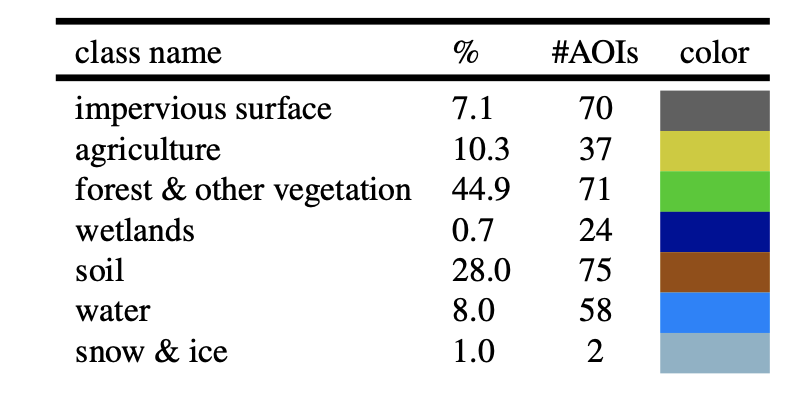
\includegraphics[width=0.5\linewidth]{LULC.png}
\end{figure}
\end{itemize}
No single AOI contains all 7 classes.\\
For a given time series, label:
$$y\in \{0,\dots, 6\}^{T\times H \times W}$$
\end{frame}

\begin{frame}{Challenges}
\begin{description}
    \item[Issue 1] Voluminous data (hundreds of GB)
    \item[Issue 2] Slow to move all images to a single processing server
\end{description}
\end{frame}

%------------------------------------------------
\section{Motivation for Federated Learning}
%------------------------------------------------

\begin{frame}{Why Federated Learning is relevant?}
\begin{description}
    \item[Solution Issue 1] client $\to$ smaller dataset $\&$ own stat. heterogeneity with clear interpretation
    \item[Solution Issue 2] No exchange of raw datasets, just each client's updates
\end{description}
\begin{itemize}
    \item Each AOI $\to$ local phenomena
    \item FL: adapt to local distrib and aggregate knowledge for better generalization
\end{itemize}
\begin{description}
    \item[$\star$ Idea 1] one AOI $=$ one client $\to$ too many clients (75);
    \item[$\star$ Idea 2] create clients based on dominant LULC categories across AOI
    \begin{enumerate}
        \item Urban areas
        \item Agricultural areas
        \item Forest-dominated areas
        \item Water-dominated areas
        \item Mixed land-use areas
    \end{enumerate}
\end{description}
\end{frame}

\begin{frame}{Federated Learning Overview}
\centering
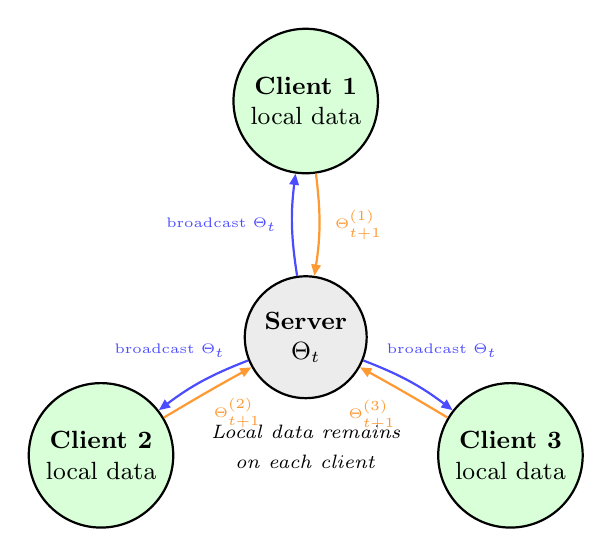
\begin{tikzpicture}[
  >=stealth,
  font=\small,
  node distance=1.2cm,
  box/.style={draw, thick, circle, minimum size=1.2cm, align=center, fill=white},
  arrowS/.style={->, thick, blue!70, arrows={-Triangle[angle=45:2pt 3]}},
  arrowC/.style={->, thick, orange!80, arrows={-Triangle[angle=45:2pt 3]}}
]

% Central server
\node[box, fill=gray!15] (server) at (0,0) {\textbf{Server} \\ $\Theta_t$};

% Three clients around server (an approximate equilateral triangle)
\node[box, fill=green!15] (client1) at (0, 3) {\textbf{Client 1}\\ local data};
\node[box, fill=green!15] (client2) at (-2.6, -1.5) {\textbf{Client 2}\\ local data};
\node[box, fill=green!15] (client3) at (2.6, -1.5) {\textbf{Client 3}\\ local data};

% Server -> Clients (blue) with slight curvature
\draw[arrowS] (server) to[bend left=8] 
   node[midway, left=4pt, align=left, xshift=2pt]{\tiny broadcast $\Theta_t$}
   (client1);
\draw[arrowS] (server) to[bend right=8]
   node[midway, above left=-1pt, align=center, xshift=0.4cm, yshift=0.2cm]{\tiny broadcast $\Theta_t$}
   (client2);
\draw[arrowS] (server) to[bend left=8]
   node[midway, above right=-1pt, align=center, xshift=-0.4cm, yshift=0.2cm]{\tiny broadcast $\Theta_t$}
   (client3);

% Clients -> Server (orange) with opposite curvature
\draw[arrowC] (client1) to[bend left=8] 
   node[midway, right=2pt, align=center]{\tiny $\Theta_{t+1}^{(1)}$}
   (server);
\draw[arrowC] (client2) to[bend left=1]
   node[midway, below right=-2pt, align=center]{\tiny $\Theta_{t+1}^{(2)}$}
   (server);
\draw[arrowC] (client3) to[bend right=1]
   node[midway, below left=-1pt, align=center]{\tiny $\Theta_{t+1}^{(3)}$}
   (server);

\node[below=0.2cm of server, text width=3.5cm, align=center] 
    {\scriptsize \textit{Local data remains on each client}};
\end{tikzpicture}

\end{frame}



\begin{frame}{Framework}
$K$ clients. Each client $k$ has dataset $D_k$ of $n_k$ pixel annotation pairs $\{x_{i}^{(k)},y_{i}^{(k)}\}_{i=1,\dots, n_k}$, where
\begin{itemize}
    \item $x_{i}^{(k)}$ is a covariance matrix in $\mathbb{R}^{4T \times 4T}$ (with $T=31$),
    \item $y_i^{(k)}\in \{0,\dots, 6\}$ is a semantic mask
\end{itemize}

\begin{description}
\item[Total number of samples] $n:=\sum_{k=1}^{K}n_k$
\item[Loss function] $\ell$ (CE) 

\item[Forward pass] SPD-Net $f_{\Theta}(\cdot)$ 
\end{description}

\centering
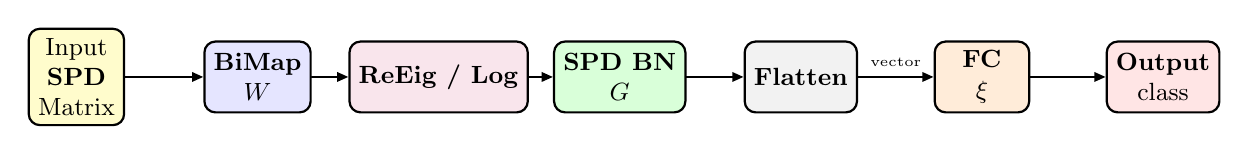
\begin{tikzpicture}[
    >=stealth,
    font=\small,
    node distance=2.3cm,
    layer/.style={draw, thick, rounded corners, align=center,
                  minimum height=0.9cm, minimum width=1.2cm, fill=white},
    arrow/.style={->, thick, line cap=round, line join=round, arrows={-Triangle[angle=45:2pt 3]}}
]

% 1) Input SPD
\node[layer, fill=yellow!20] (input) {Input\\\textbf{SPD}\\ Matrix};

% 2) BiMap(W)
\node[layer, fill=blue!10, right of=input] (bimap) {\textbf{BiMap}\\ $W$};
\draw[arrow] (input) -- (bimap) 
   node[midway,below,align=center]{};

% 3) ReEig/Log
\node[layer, fill=purple!10, right of=bimap] (re) {\textbf{ReEig / Log}};
\draw[arrow] (bimap) -- (re);

% 4) BN(G)
\node[layer, fill=green!15, right of=re] (bn) {\textbf{SPD BN}\\$G$};
\draw[arrow] (re) -- (bn);

% 5) Flatten
\node[layer, fill=gray!10, right of=bn] (flatten) {\textbf{Flatten}};
\draw[arrow] (bn) -- (flatten);

% 6) FC(xi)
\node[layer, fill=orange!15, right of=flatten] (fc) {\textbf{FC}\\$\xi$};
\draw[arrow] (flatten) -- (fc) node[midway,above]{\tiny vector};

% 7) Output
\node[layer, fill=red!10, right of=fc] (output) {\textbf{Output}\\class};
\draw[arrow] (fc) -- (output);

% optional note
%\node[below=0.2cm of flatten, text width=2.7cm, align=center]{\scriptsize \textit{...}};
\end{tikzpicture}
\end{frame}
\begin{frame}

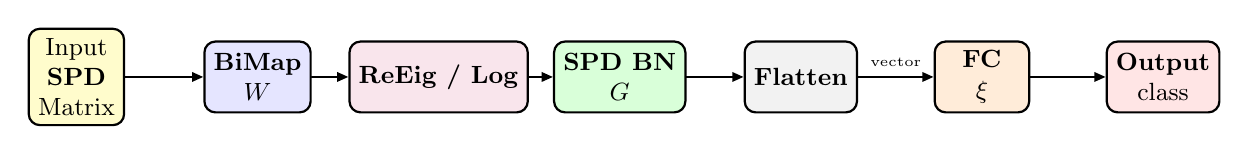
\begin{tikzpicture}[
    >=stealth,
    font=\small,
    node distance=2.3cm,
    layer/.style={draw, thick, rounded corners, align=center,
                  minimum height=0.9cm, minimum width=1.2cm, fill=white},
    arrow/.style={->, thick, line cap=round, line join=round, arrows={-Triangle[angle=45:2pt 3]}}
]

% 1) Input SPD
\node[layer, fill=yellow!20] (input) {Input\\\textbf{SPD}\\ Matrix};

% 2) BiMap(W)
\node[layer, fill=blue!10, right of=input] (bimap) {\textbf{BiMap}\\ $W$};
\draw[arrow] (input) -- (bimap) 
   node[midway,below,align=center]{};

% 3) ReEig/Log
\node[layer, fill=purple!10, right of=bimap] (re) {\textbf{ReEig / Log}};
\draw[arrow] (bimap) -- (re);

% 4) BN(G)
\node[layer, fill=green!15, right of=re] (bn) {\textbf{SPD BN}\\$G$};
\draw[arrow] (re) -- (bn);

% 5) Flatten
\node[layer, fill=gray!10, right of=bn] (flatten) {\textbf{Flatten}};
\draw[arrow] (bn) -- (flatten);

% 6) FC(xi)
\node[layer, fill=orange!15, right of=flatten] (fc) {\textbf{FC}\\$\xi$};
\draw[arrow] (flatten) -- (fc) node[midway,above]{\tiny vector};

% 7) Output
\node[layer, fill=red!10, right of=fc] (output) {\textbf{Output}\\class};
\draw[arrow] (fc) -- (output);

% optional note
%\node[below=0.2cm of flatten, text width=2.7cm, align=center]{\scriptsize \textit{...}};
\end{tikzpicture}
Each client's SPD-net with $L$ layers has learnable parameters
$$\Theta=(\underbrace{W_1,\dots, W_{L}}_{BiMap}, \underbrace{G_1,\dots, G_{L}}_{BN},\underbrace{\xi_1,\dots,\xi_{d}}_{FC}) \in \mathcal{M}$$
with 
$$\mathcal{M}:=\left(\prod_{l=1}^{L} \text{St}(d_{l},d_{l+1})\right) \times \left(\prod_{l=1}^{L}\text{SPD}_{d_l}\right) \times \mathbb{R}^{d}.$$

\end{frame}

\begin{frame}
\begin{description}
    \item[Local objective functions] For each client $k=1,\dots, K$,
    $$F_k(\Theta):=\frac{1}{n_k}\sum_{i=1}^{n_k}\ell\bigl(f_{\Theta}(x_i^{(k)}),\,y_i^{(k)})\bigr).$$
    \item[Global objective function]
    $$\arg \min_{\Theta \in \mathcal{M}}F(\Theta):=\sum_{k=1}^{K}\frac{n_k}{n}\,F_k(\Theta).$$
\end{description}
\end{frame}

%------------------------------------------------
\section{Federated Procedure}
%------------------------------------------------

\begin{frame}{Federated procedure}
\begin{block}{Algorithm}
\begin{description}
    \item[$\star$ \textbf{Initialization}] $\Theta_{0}$ to all clients (random)
    \item[$\star$ \textbf{Outer loop}] For $t=0,\dots, T-1$ (rounds):
    \begin{enumerate}
        \item A subset $\mathcal{S}_t$ of $r\leq K$ clients is sampled (random)
        \item Server broadcasts $\Theta_{t}$ to clients.
        \item Each client $k\in \mathcal{S}_t$ runs $E_k$ local updates on $\Theta$ with initialization $\Theta_{t}$.
        \item Aggregation of each client's local updated parameters via barycenters $\to$ $\Theta_{t+1}$
    \end{enumerate}
    \item[$\star$ \textbf{Global output}] Final aggregated param. $\Theta_{T}$ or $\text{Unif}(\{\Theta_{0},\dots,\Theta_{T}\})$
\end{description}
\end{block}
\vspace{0.5cm}
If each local function $F_k$ is $L_k$-smooth and geodesically convex, then the algorithm converges in $O(1/T)$ (provided some curvature/manifold additional assumptions).
\end{frame}

%------------------------------------------------
\subsection{Riemannian local optimization}
\begin{frame}{Riemannian local updates at client $k\in \mathcal{S}_r$}
Let $\theta$ denote a Riemannian parameter (either one of the $W_l$ or $G_l$).  
\begin{itemize} 
\item Initialize $\theta_0^{(k)}=\theta_{t}$
\item For $s=1,\dots, E_k$:
    \[
      \theta_{s+1}^{(k)} \;=\; R_{\theta_{s}^{(k)}}\Bigl(-\eta^{(k)}\, g^{(k)} \Bigr),
    \]
    where the local Riemannian gradient is
    \[
      g^{(k)} \;=\; \text{grad}\, F_k\!\bigl(\theta_s^{(k)}\bigr)
      \;\;\textcolor{blue}{-\;\mathcal{T}_{\,\theta_{t}\to \theta_s^{(k)}}\Bigl(\text{grad}\, F_k(\theta_t)\;-\;\text{grad}\, F(\theta_t)\Bigr)},
    \]
    \begin{itemize}
      \item The \textcolor{blue}{blue} term is the optional \textbf{SVR correction} (variance reduction).
    \end{itemize}
\end{itemize}
\end{frame}

%------------------------------------------------
\subsection{Differential Privacy Option}
%------------------------------------------------

\begin{frame}{Differential Privacy as a model variant}
Besides the \textcolor{blue}{variance-reduction} approach, we can also inject 
\textcolor{dpColor}{\textbf{DP noise}} on each local gradient to protect sensitive data.  
\vspace{1ex}

\textbf{Key idea:} Add tangent-space Gaussian noise before retraction/exponential update.

\begin{itemize}
  \item \textcolor{dpColor}{\textbf{DP}} can be combined with or without the 
   \textcolor{blue}{SVR} term.
  \item Each client $k$ ensures local DP by perturbing its gradient:
  \[
     g_{\text{DP}}^{(k)} 
     \;=\; 
     g^{(k)} \;\; \textcolor{dpColor}{+\;\varepsilon_t},
     \quad \text{where} \quad
     \varepsilon_t \;\sim\; \mathcal{N}_{\,\theta_s^{(k)}}\bigl(0,\sigma^2\bigr).
  \]
  \item This noise is drawn from a \emph{tangent-space Gaussian} distribution 
    at $\theta_s^{(k)}$.
\end{itemize}

\textcolor{dpColor}{\textbf{Privacy Guarantee:}}
With an appropriate choice of $\sigma$ and composition rules, the entire FL pipeline can provide an $(\varepsilon,\delta)$-DP guarantee.
\end{frame}

\begin{frame}{Riemannian local updates with optional DP}
\begin{itemize} 
\item Initialize $\theta_0^{(k)}=\theta_{t}$
\item For $s=1,\dots, E_k$:
    \[
      g^{(k)} \;=\; \text{grad}\,F_k\!\bigl(\theta_s^{(k)}\bigr)
                \;\;\textcolor{blue}{-\;\mathcal{T}_{\,\theta_{t}\to \theta_s^{(k)}}
                \Bigl(\text{grad}\, F_k(\theta_t)\;-\;\text{grad}\, F(\theta_t)\Bigr)},
    \]
    \[
      \textcolor{dpColor}{g_{\text{DP}}^{(k)} \;=\; g^{(k)} \;+\;\varepsilon_s,
      \qquad \varepsilon_s \;\sim\; \mathcal{N}_{\,\theta_s^{(k)}}(0,\sigma^2).}
    \]
    Then update via retraction (or exponential map):
    \[
      \theta_{s+1}^{(k)} \;=\; R_{\theta_{s}^{(k)}}\Bigl(-\eta^{(k)}\, \textcolor{dpColor}{g_{\text{DP}}^{(k)}}\Bigr).
    \]
    \begin{itemize}
      \item \textcolor{dpColor}{\textbf{Red}} term is the \textbf{DP noise} addition (optional)
      \item \textcolor{blue}{\textbf{Blue}} term is still the \textbf{SVR correction} (optional).
    \end{itemize}
\end{itemize}
\end{frame}
\subsection{Euclidean local optimization}
\begin{frame}{Local updates for Euclidean FC weights (SVR + DP)}
Let $\xi \in \mathbb{R}^{d_{\mathrm{FC}}}$ be the parameter vector for the final fully-connected layer.  
During each local epoch on client $k$:
\[
   \xi_{0}^{(k)} \;=\; \xi_{t}, 
\quad
   \text{and for }\, s=0,\dots,E_k-1:\]
   \[
   \xi_{s+1}^{(k)} 
   \;=\; 
   \xi_{s}^{(k)} 
   \;-\;
   \eta^{(k)}\,
   \Bigl(\nabla F_{k}\bigl(\xi_{s}^{(k)}\bigr)
     \;\textcolor{blue}{-\;\bigl[\nabla F_{k}(\xi_{t})-\nabla F(\xi_{t})\bigr]}
     \;+\;\textcolor{dpColor}{\varepsilon_{s}}\Bigr),
\]
where:
\begin{itemize}
  \item $\nabla F_{k}(\xi_{s}^{(k)})$: local Euclidean gradient on client $k$.
  \item \(\textcolor{blue}{\bigl[\nabla F_{k}(\xi_{t}) - \nabla F(\xi_{t})\bigr]}\) is the \textbf{SVR correction} term.
  \item \(\textcolor{dpColor}{\varepsilon_{s}}\sim \mathcal{N}(0,\,\sigma^2 I)\) is the \textbf{DP noise} term.
  \item After $E_k$ steps, client $k$ sends $\xi_{E_k}^{(k)}$ to the server.
\end{itemize}

\end{frame}

%------------------------------------------------
\section{Server Aggregation}
%------------------------------------------------
\subsection{Riemannian aggregation}
\begin{frame}{Server aggregation (Karcher flow) for $\theta=G$ SPD}
After each client $k \in \mathcal{S}_r$ sends back $\theta_{E_k}^{(k)}$, we compute the Riemannian (Fréchet) mean on the manifold:
\[
  \Theta_{t+1} \;=\; 
    \arg\min_{\Theta\in\mathcal{M}} \;\sum_{k\in \mathcal{S}_r} p_k\,d\bigl(\Theta,\;\theta_{E_k}^{(k)}\bigr)^2.
\]
\begin{itemize}
\item In practice, we use a gradient-descent-based procedure (Karcher flow):
\[
   \Theta_{t+1} 
   \;\leftarrow\; 
   \mathrm{Exp}_{\Theta_{t}}\!\Bigl(\,-\,\gamma\sum_{k\in \mathcal{S}_r} 
   p_k\,\mathrm{Log}_{\Theta_{t}}(\theta_{E_k}^{(k)})\Bigr),
\]
where $\gamma$ is a step size for the Karcher flow.
\end{itemize}

\end{frame}

%------------------------------------------------



\begin{frame}{Server aggregation (projection-based) for \(\mathbf{W}\in \mathrm{St}(d_l,d_{l+1})\)}
For the BiMap parameters \(W_l\) living on the Stiefel manifold, we can use:

\begin{itemize}
    \item \textbf{Karcher flow} or Riemannian gradient-based aggregator: 
    \[
      W_{t+1}
      \;=\;
      \arg\!\min_{W\in \mathrm{St}(d_l,d_{l+1})}
      \sum_{k\in S_t} p_k\,d^2\bigl(W,\,W_{\tau}^{(k)}\bigr),
    \]
    which can be iteratively approximated (exp/log maps).
    \item \textbf{Projection-based aggregator}:
    \[
      W_{t+1}
      \;=\; \mathrm{uf}\!\Bigl(\underbrace{\sum_{k\in S_t}p_k\,W_{\tau}^{(k)}}_{\text{arithmetic mean}}\Bigr)
      \quad\text{or}\quad
      W_{t+1}
      \;=\; \mathrm{qf}\!\Bigl(\sum_{k\in S_t}p_k\,W_{\tau}^{(k)}\Bigr).
    \]
     No iterative scheme needed, computationally cheaper (simple retractions/liftings).
\end{itemize}
\end{frame}
%===============================================================
\subsection{Euclidean aggregation}
%===============================================================


\begin{frame}{Server aggregation of FC weights}
At round $t$, we receive each client’s updated $\xi_{E_k}^{(k)}$ for $k \in \mathcal{S}_t$.  
To get $\xi_{t+1}$,  standard weighted average (FedAvg):
\[
   \xi_{t+1}
   \;=\; \sum_{k\in \mathcal{S}_t} \, \frac{n_k}{\sum_{j\in \mathcal{S}_t}n_j}\,\xi_{E_k}^{(k)}
\]

\vspace{.5em}

No need for any Riemannian retraction or manifold-based aggregator.  
\end{frame}

%------------------------------------------------
\begin{frame}{References}
\tiny
\bibliography{reference.bib}
\bibliographystyle{apalike}
\end{frame}

\end{document}

